\subsection{Example of use of ART Editor: The NURE Use Case}
\label{subsec:art-editor-nure-example}

In the previous \autoref{ch:conceptual-model}, we applied the XRM Conceptual Model to a real case study provided by the company Fifthingenium. Since the model proved to be very effective in describing the experience, we decided to represent NURE also by using the ART Editor. 
As in \autoref{sec:conceptual-nure-example}, we are only modelling an extract of the inner journey for obvious reasons of space. 
Consider also that between the case study modelled with the XRM and the one using the Editor there are some semantic differences for which we refer to \autoref{subsec:art-editor-from-conceptual}.

\subsection*{Elements}

Below are the elements that are part of the excerpt from the NURE experience associated with the corresponding default elements of the ART Editor.

\begin{itemize}
    \item 3D Scene: The 3D Scene element has been used to distinguish the different scenes of the whole experience. Each scene corresponds to an Augmented Environment in the XRM Model. Respectively, AE 2 corresponds to "Scene 1", AE 2.2 to "Scene 2" and AE 3 to "Scene 3". In addition, "Scene 1" is also inserted here, since the ART Editor is based on the concepts of State-Action-Effect and therefore requires an initial state.
    \item 3D Object: The 3D Object element represents the Static Objects of the XRM Model, exactly the Tomb D, the Tomb E, the respective covering slabs, the interior and the exterior of the Mausoleum.
    \item 3D Video: The 3D Video element, corresponding to a Dynamic Object in the XRM Model, represents the reproducible scene of the ancient Refrigerium ritual.
    \item QR Code: The QR Code element corresponds to an Interaction Placeholder in the XRM Model and provides the user with an alternative to trigger a new scene.
    \item Menu: The Menu element is represented by a Button, an Operational Object, in the XRM Model and provides the user with an alternative to trigger a new scene.
\end{itemize}

\subsection*{Use Case Scenario}

Once again, it was decided to explain in detail the modelling built using the ART Editor through the use of a use case scenario, this time adopting the point of view of a user, an art curator and designer, who uses our Editor. 

Laura is 31 years old, studied Economics and Management of Arts and Cultural Activities at Ca' Foscari in Venice and now she works in an agency that deals with the design, curatorship and exhibition of cultural and artistic events. Laura received a proposal from the cultural organisation NURE which asked her to design an extended reality experience in the archaeological area of Santa Lucia di Assolo (OR) in Sardinia.

Although the idea is very exciting, Laura fears she does not have the right skills to use XR frameworks or to interact with the engineering team. After learning about the existence of the ART Editor, Laura starts to imagine the NURE experience, so she decides to compose it. After receiving the requirements and the media provided by the archaeological area authority, she can launch the Editor, which presents on the right the list of elements needed to build the experience. 

Laura decides to design the most interesting area of the whole path (\autoref{fig:nure1}, \autoref{fig:nure2}) , the one that starts from Scene 2, therefore she provides the user with a double alternative to activate Scene 2, that is by tapping on Menu2 or simply letting the user move away from Scene 1 to get closer to Scene 2.

In both cases all components of scene 2, such as Tomb D, Tomb E, the respective covering slabs, the outside of the Mausoleum are visible, except for the inside of the Mausoleum. Laura wants the 3D models to be appealing, to stimulate the visitor to interact with them, so she inserts as State Tag the Blinking, a luminous outline for each model. 
As the models are placed at progressive distances, Laura wants to give the visitor the possibility to be free to choose what to interact with first. She knows that XR experiences are dynamic experiences, where the user is encouraged to continue at a certain pace in the designed path, for several reasons including the limited battery life of the Visors. 

Moreover, she decides to insert the Swipe as an Action Tag, so that the user can slide with the finger on the slabs of the tombs to see the inside, since the covers have become transparent. Once past the tombs, Laura wants the user to see the centrepiece of this Scene, in fact when the user moves away, the tombs become hidden and through the menu the user can activate Scene 2.2, which also includes the Interior of the Mausoleum. 

Laura, has left the outside of the Mausoleum still visible and blinking but with 50\% opacity, allowing a glimpse of something inside. The user is thus encouraged to tap on the outside of the Mausoleum, to see the inside. 

Our designer decides to start the 3D video of the Refrigerium scene at the end of a 5-second timer. Once the video is over, the user can activate scene 3, again with a double option, by framing the QR code or using Menu3 of the application. 

Laura is very satisfied with her design, especially because it was easy and very intuitive to use the ART Editor. Now all she has to do is generate the JSON file and and submit it to the HMD application to complete the development of the experience.

\begin{figure}[h]
    \centering
    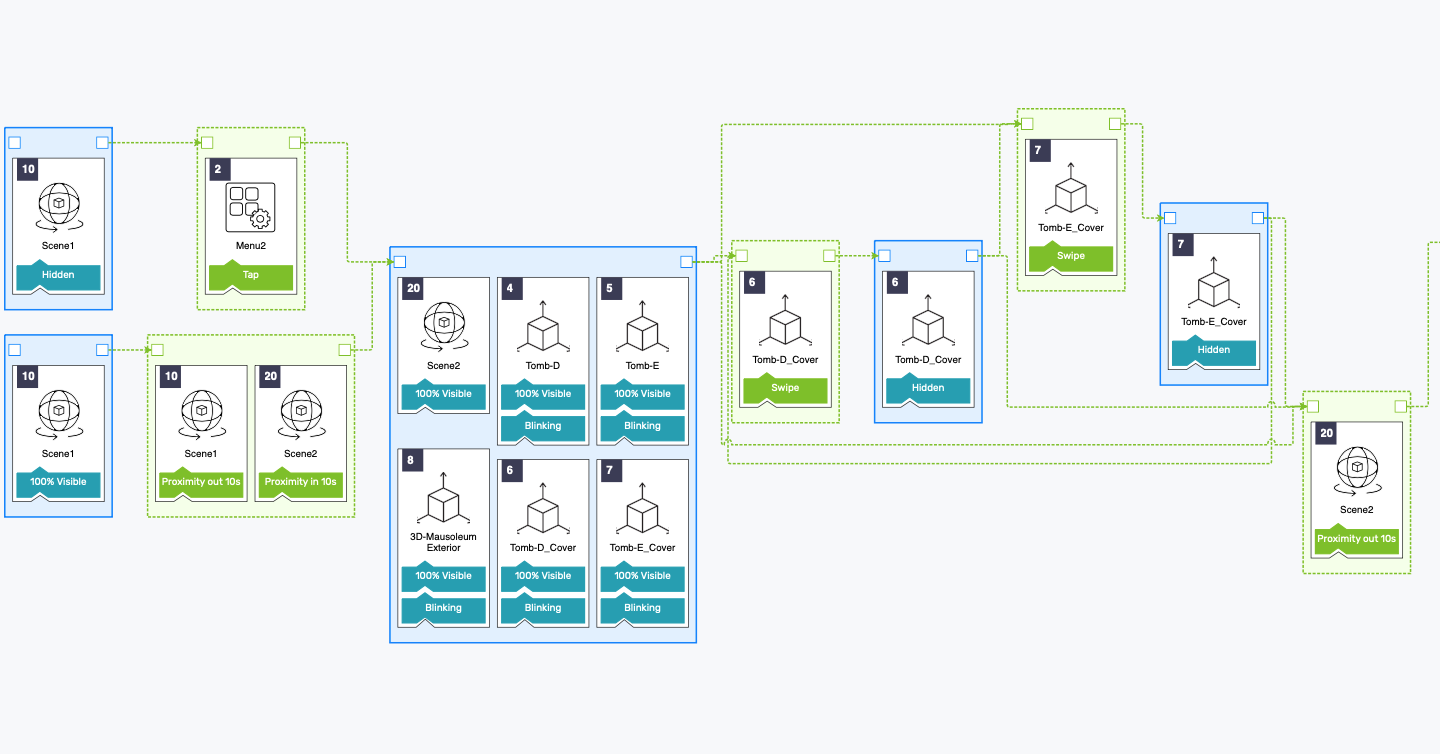
\includegraphics[width=\linewidth]{Figures/Editor/nure/NureExample1.png}
    \caption{ART Case Study 1st part - NURE}
    \label{fig:nure1}
\end{figure}

\begin{figure}[h]
    \centering
    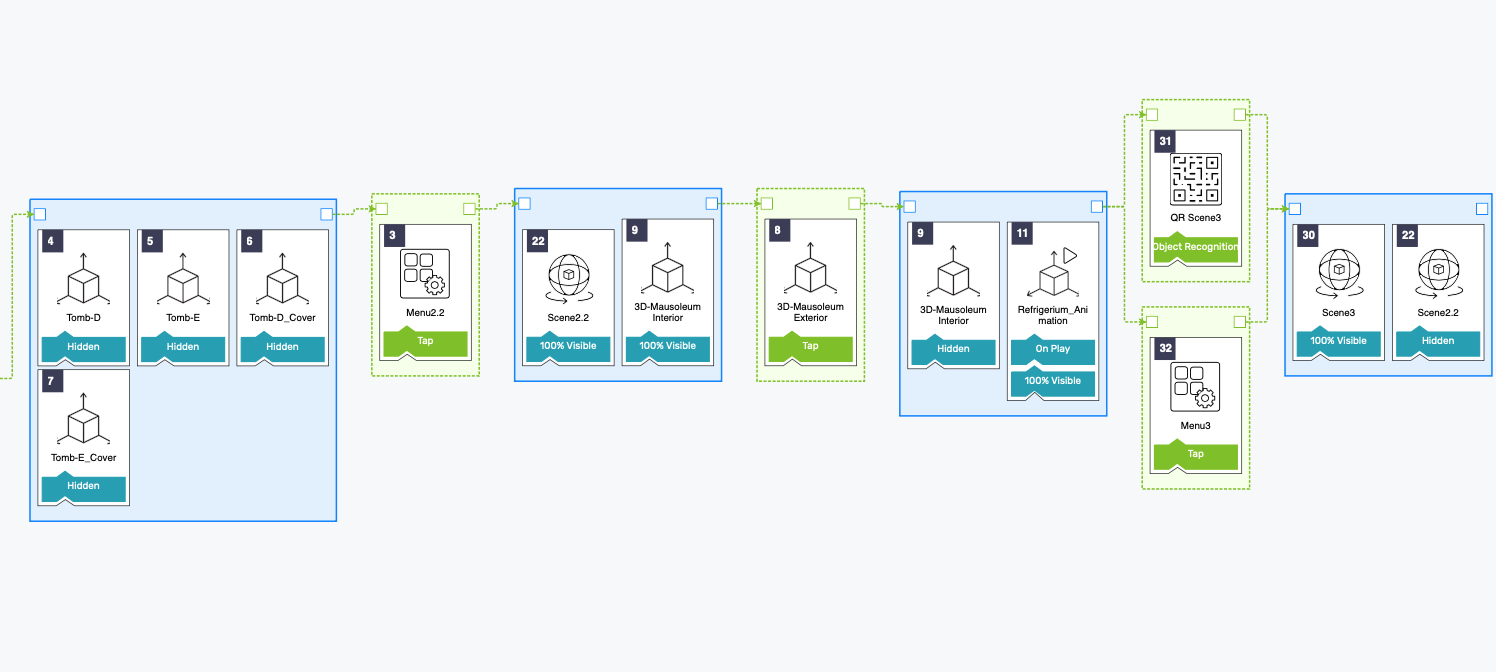
\includegraphics[width=\linewidth]{Figures/Editor/nure/NureExample2.png}
    \caption{ART Case Study 2nd part - NURE}
    \label{fig:nure2}
\end{figure}